% No modificar estas líneas de código, por favor dirigirse a MARCO TEÓRICO

\newpage

%------------------------
%
%       MARCO TEÓRICO
%
%------------------------

\section{MARCO TEÓRICO}
 En el presente capítulo se revisan los conceptos necesarios a ser utilizados en el desarrollo del proyecto. Primeramente, como base del proyecto, se define el concepto de autoclave y su principio de funcionamiento; los modelos de mantenimiento que existen y finalmente, se hace un desglose de las tecnologías a usar.
 
\subsection{Fundamentos de las autoclaves}
De acuerdo a \cite{autoclave} `` Un autoclave es un dispositivo metálico con una cámara de cierre hermético que se utiliza para realizar procesos de esterilización empleando vapor de agua a alta presión. Principalmente son empleados en la industria médica para la esterilización de instrumentos quirúrgicos '' 

Los autoclaves son esenciales en la esterilización médica porque eliminan todos los microorganismos, incluyendo bacterias, virus y esporas. Mantener las condiciones adecuadas de temperatura y presión es crucial para asegurar que los instrumentos quirúrgicos estén completamente esterilizados y seguros para su uso en pacientes. La presencia de agentes bacterianos en los instrumentos puede llevar a infecciones graves, por lo que la esterilización adecuada es parte fundamental en el control de infecciones en entornos médicos \citep{autoclave2}.

\subsubsection{Principio de funcionamiento}

El ciclo de esterilización está formado por tres etapas; una etapa inicial en la cual se somete al material tratado a un determinado valor de presión negativa; una segunda etapa en la cual el material debe alcanzar un valor fijo de temperatura, mediante la inyección de vapor dentro del recipiente que lo contiene durante un determinado tiempo; y finalmente, una tercera etapa en la que se somete nuevamente al material a un determinado valor de presión negativa durante cierto tiempo \citep{funcionamiento}.

De acuerdo con \cite{funcionamiento}, una vez cumplidas estas etapas, se dice que el material tratado ya está estéril y libre de cualquier bacteria y microorganismo para ser manipulado en el área de la industria médica.

\begin{figure}[!htb]
   \centering
   \caption{Principio de funcionamiento del autoclave}
   {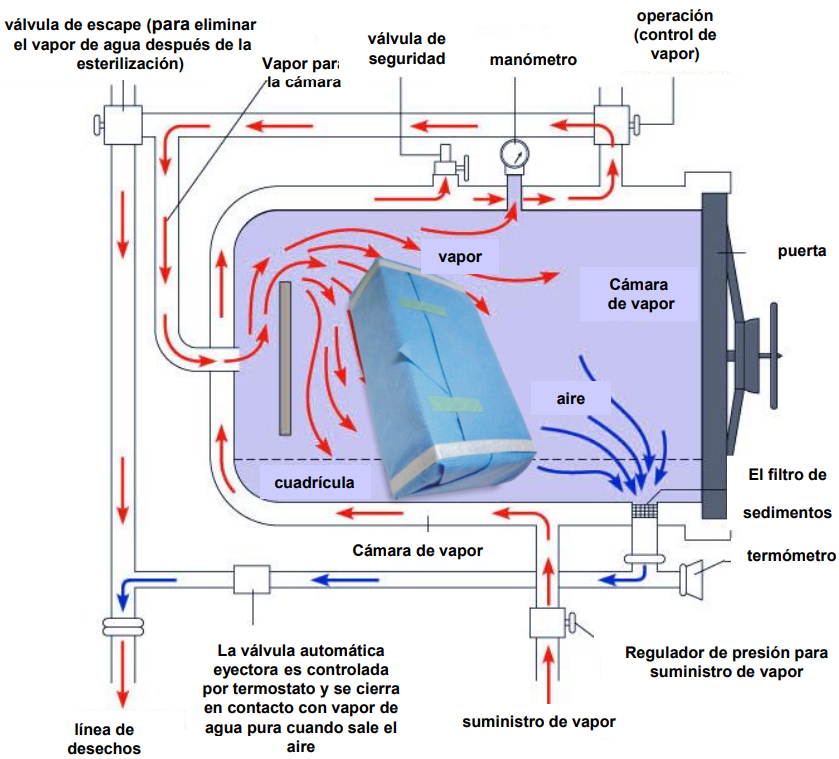
\includegraphics[scale=0.8]{Figuras/autoclave.png}}\\
    \centering{\textbf{Fuente:} Apuntes de electromecánica Xavier Pardell}
\end{figure}

\paragraph{Tratamiento previo}
Para lograr una esterilización efectiva con vapor, es esencial la presencia de humedad, ya que esta permite que el vapor llegue directamente a los microorganismos que se desean eliminar; cualquier resto de aire actúa como aislante, reduciendo la eficacia y temperatura del proceso. La fase de pretratamiento consiste en variar la presión para eliminar el aire de las cargas a esterilizar y generar la humedad necesaria, asegurando siempre el cierre hermético de la puerta del autoclave antes de iniciar la esterilización \citep{funcionamiento2}.

\paragraph{Esterilización}
En esta fase, es crucial ajustar adecuadamente las temperaturas tanto de la cámara como de la camisa del autoclave (la camisa es una capa externa que rodea la cámara, diseñada para distribuir el calor de forma uniforme). También es importante permitir que pequeñas cantidades de vapor escapen de la cámara al exterior, ya que esto ayuda a eliminar cualquier residuo de aire y condensado. La temperatura del vapor, que coincide con la temperatura de la cámara, debe ser medida y registrada.

Una vez que se alcanza la temperatura predeterminada para la esterilización, se inicia el conteo del tiempo necesario, durante el cual la temperatura no debe descender por debajo del nivel establecido. En otras palabras, se debe mantener constante la temperatura configurada dentro de la cámara durante toda esta fase, asegurando además que la puerta del autoclave permanezca sellada herméticamente \citep{funcionamiento2}.

\paragraph{Tratamiento final}
De acuerdo con \cite{funcionamiento} esta etapa tiene como objetivo equilibrar la temperatura y humedad de las cargas a esterilizar. Para lograr esto, se reduce la presión dentro de la cámara a niveles inferiores a la presión atmosférica, creando un vacío. Luego, se introduce aire filtrado en la cámara para restablecer gradualmente la presión atmosférica. Una vez alcanzada, se desbloquea el cierre hermético de la puerta del autoclave, permitiendo retirar la carga esterilizada y restaurar las condiciones iniciales para iniciar un nuevo ciclo de esterilización.

\subsubsection{Tipos de autoclaves}
Existen distintos tipos de autoclaves, cada uno diseñado para diferentes aplicaciones y necesidades específicas de esterilización; en la siguiente sección mencionamos algunas:
 
\paragraph{Autoclaves de vacío previo}
De acuerdo con \cite{medina} las autoclaves de vacío previo utilizan una bomba de vacío para extraer el aire de la cámara antes de introducir vapor, lo que permite una esterilización más efectiva de materiales porosos y con cavidades, al garantizar que el vapor penetre adecuadamente. Este proceso elimina el aire residual que podría actuar como aislante, asegurando una distribución uniforme del calor y la humedad. Son comúnmente usadas en hospitales y laboratorios para esterilizar instrumentos médicos complejos y cargas de difícil acceso.

\paragraph{Autoclaves de alta velocidad }
Para \cite{altavelocidad} esta autoclave combina el vacío previo con altas temperaturas, permitiendo ciclos de esterilización más rápidos. Son ideales para hospitales o laboratorios que requieren una rápida esterilización de instrumentos.

\paragraph{Autoclaves de sobremesa}
Las autoclaves de sobremesa son modelos compactos y de menor capacidad, diseñados para esterilizar equipos pequeños, instrumentos y materiales en entornos con espacio limitado, como clínicas, laboratorios y consultorios. A pesar de su tamaño, ofrecen un alto rendimiento en la esterilización, utilizando vapor a alta presión para garantizar la eliminación de microorganismos. Estas autoclaves son ideales para esterilizar pequeños lotes de instrumentos médicos, vidrio, medios de cultivo y otros materiales, siendo una opción eficiente para lugares con necesidades moderadas de esterilización \citep{demesa}.

\begin{figure}[!htb]
   \centering
   \caption{Autoclave Industrial}
   {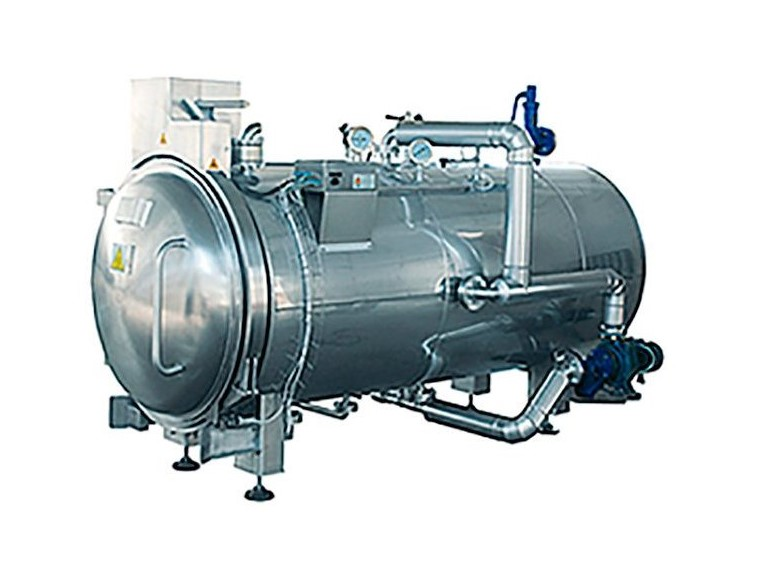
\includegraphics[scale=0.5]{Figuras/esterilizador.jpg}}\\
    \centering{\textbf{Fuente:} MECAL S.A.}
\end{figure}


\paragraph{Autoclaves industriales}
Son de gran tamaño y están diseñados para la esterilización a gran escala en entornos industriales, como en la producción de alimentos en conserva, la industria farmacéutica y otras aplicaciones de manufactura \citep{garcia_autoclave_industrial_2018}

\subsubsection{Relevancia del mantenimiento de autoclaves}
El mantenimiento adecuado de los autoclaves es esencial para asegurar su operación segura y eficiente, ya que estos equipos son vitales en la esterilización de instrumentos y materiales en sectores como el médico y farmacéutico. Si un autoclave no recibe el mantenimiento necesario, pueden ocurrir fallos en el control de la temperatura y la presión, lo que afectaría la efectividad de la esterilización y podría causar la contaminación de los equipos o productos. Además, el deterioro de sus componentes puede representar riesgos de seguridad, como fugas de vapor o fallos en el cierre hermético, lo que podría ocasionar accidentes o daños a los materiales sometidos al proceso \citep{Relevancia}.


Segun \cite{Relevancia} mantenimiento preventivo regular permite identificar y corregir problemas antes de que se conviertan en fallas graves, lo que extiende la vida útil del equipo y reduce costos operativos a largo plazo. La inspección de componentes como válvulas, sensores, bombas de vacío y sistemas de calefacción es esencial para asegurar que el autoclave opere dentro de los parámetros establecidos. Además, el monitoreo continuo del estado del equipo, mediante sistemas de monitoreo remoto o pruebas de funcionamiento, puede detectar anomalías tempranas y facilitar un mantenimiento más eficiente, mejorando la confiabilidad del proceso de esterilización.

\subsubsection{Estándares y normativas}
Los estándares y normativas para autoclaves son fundamentales para garantizar que estos equipos de esterilización operen de manera segura y efectiva en diversos sectores industriales, especialmente en los ámbitos médico, farmacéutico y alimentario. Estas normativas regulan tanto los requisitos de diseño y construcción de los autoclaves, como los procedimientos operativos y de mantenimiento, asegurando que los equipos cumplan con los estándares de seguridad, eficacia y calidad. Uno de los principales estándares internacionales en este campo es la norma ISO 13485, que establece los requisitos para los sistemas de gestión de calidad de dispositivos médicos, incluyendo los autoclaves utilizados en la esterilización de instrumentos médicos  \citep{iso_13485_2016}.

Además de las normativas internacionales, existen regulaciones locales y regionales que pueden variar según el país o la región. Por ejemplo, en los Estados Unidos, la Administración de Alimentos y Medicamentos (FDA) establece regulaciones específicas para los autoclaves utilizados en la esterilización de dispositivos médicos, garantizando que estos equipos cumplan con los estándares de seguridad y eficiencia. En la Unión Europea, la Directiva de Dispositivos Médicos (93/42/EEC) regula los requisitos de los autoclaves, asegurando que estén marcados con el sello CE, lo que indica que cumplen con los requisitos de seguridad y rendimiento de la región \citep{fda_autoclaves_2020}.

En cuanto a las pruebas de funcionamiento, las normativas también exigen que los autoclaves sean sometidos a verificaciones periódicas para asegurar su efectividad en la esterilización. Esto incluye pruebas de temperatura, presión y ciclos de esterilización, además de la validación del proceso, para verificar que los equipos mantengan las condiciones necesarias para la eliminación completa de microorganismos. Los procedimientos de mantenimiento y calibración deben estar bien documentados y seguir procedimientos específicos para prevenir fallas y garantizar el rendimiento óptimo del autoclave durante su vida útil, lo que es vital para la seguridad de los productos y materiales procesados.

\subsection{Modelos de mantenimiento}

El mantenimiento industrial incluye diferentes enfoques o modelos que buscan asegurar el funcionamiento continuo de los equipos y minimizar las interrupciones por fallos. Cada modelo de mantenimiento presenta ventajas y desafíos únicos, y su selección depende de factores como el tipo de equipo, el costo y los recursos disponibles.

\subsubsection{Mantenimiento correctivo}
El mantenimiento correctivo  o reactivo, consiste en una estrategia de gestión que se aplica después de que un equipo o sistema presenta una falla o interrupción en su funcionamiento. Su principal objetivo es restaurar la operatividad del equipo mediante reparaciones o reemplazos necesarios. Según \cite{Mobley2002}, este tipo de mantenimiento es reactivo por naturaleza, ya que no se toman medidas preventivas antes de que ocurra el fallo. Aunque puede ser adecuado en equipos no críticos o cuando los costos de implementación de otros enfoques son prohibitivos, el mantenimiento correctivo tiene desventajas importantes, como tiempos de inactividad prolongados y gastos elevados en reparaciones de emergencia.

Desde una perspectiva económica, el mantenimiento correctivo es menos eficiente en comparación con estrategias como el mantenimiento preventivo o predictivo. Tal como señalan \cite{Kelly2012}, los costos derivados del tiempo de inactividad no planificado, la necesidad de mano de obra de emergencia y la adquisición urgente de repuestos pueden superar significativamente el costo inicial de implementación de estrategias preventivas. No obstante, en algunos casos, puede ser una estrategia válida para equipos de bajo valor o sistemas cuya falla no impacte significativamente las operaciones principales. Para mitigar los riesgos asociados, se recomienda combinar el mantenimiento correctivo con enfoques más proactivos que permitan anticiparse a fallos críticos.

\subsubsection{Mantenimiento preventivo}

El mantenimiento preventivo se realiza de forma programada con el objetivo de reducir la probabilidad de fallos en los equipos o sistemas. Según \cite{Mobley2002}, este enfoque implica la realización periódica de inspecciones, ajustes y reemplazos de componentes para mantener los equipos en condiciones óptimas de funcionamiento. Una de sus principales ventajas es la capacidad de minimizar los tiempos de inactividad no planificados, ya que las intervenciones se realizan de manera controlada. Además, el mantenimiento preventivo es especialmente útil en equipos críticos, donde las fallas inesperadas podrían causar interrupciones significativas en las operaciones.

Desde una perspectiva económica, el mantenimiento preventivo es más rentable a largo plazo en comparación con el mantenimiento correctivo. Tal como destaca \cite{Wireman2004}, invertir en un programa de mantenimiento preventivo bien planificado permite reducir los costos asociados con reparaciones de emergencia y pérdidas de producción. Sin embargo, esta estrategia también conlleva ciertos desafíos, como la necesidad de planificar recursos y establecer programas que no interfieran con las operaciones normales. A pesar de estos retos, el mantenimiento preventivo es ampliamente reconocido como una práctica esencial para garantizar la eficiencia y la seguridad en los entornos industriales.

\subsubsection{Mantenimiento predictivo}
Este mantenimiento se basa en el monitoreo continuo de equipos y sistemas para anticipar fallas antes de que ocurran. Según \citep{Mobley2002}), esta técnica se fundamenta en el análisis de datos recopilados a través de sensores y herramientas de diagnóstico, lo que permite identificar patrones de desgaste y predecir el momento óptimo para realizar intervenciones. A diferencia del mantenimiento preventivo, el predictivo no se realiza en intervalos fijos, sino cuando los datos indican una necesidad específica, optimizando así los recursos y el tiempo dedicado al mantenimiento. Esta estrategia es especialmente útil en entornos industriales donde el tiempo de inactividad no planificado puede tener un impacto crítico.

En términos económicos, el mantenimiento predictivo tiene el potencial de ofrecer ahorros significativos al reducir los costos asociados con reparaciones de emergencia y minimizar los tiempos de inactividad no planificados. Según \cite{Jardine2006}, esta metodología puede extender la vida útil de los equipos y mejorar la productividad general al garantizar que las intervenciones de mantenimiento se realicen solo cuando son necesarias. Sin embargo, su implementación requiere una inversión inicial considerable en tecnología, capacitación y sistemas de análisis de datos, lo que puede ser un desafío para algunas organizaciones. A pesar de estos costos iniciales, los beneficios a largo plazo en términos de eficiencia y reducción de costos operativos hacen que el mantenimiento predictivo sea una opción estratégica en la gestión moderna de activos.


\subsection{Tecnologías de IoT}
Las tecnologías de \acrfull{iot} permiten la conexión y comunicación entre dispositivos físicos a través de internet, utilizando sensores, actuadores y plataformas de gestión. Estas tecnologías recopilan, procesan y analizan datos en tiempo real para automatizar procesos, mejorar la eficiencia y tomar decisiones basadas en datos. Su aplicación esta presente en sectores como la industria, salud, transporte, por mencionar algunas.

\subsubsection{IoT y su aplicación en la industria de la salud}

La aplicación de \acrshort{iot} implica que los dispositivos recopilen, compartan y analicen datos sin intervención humana directa. Los dispositivos \acrshort{iot} están equipados con sensores, software y otras tecnologías que les permiten interactuar con su entorno y enviar información a otros sistemas para su procesamiento y análisis.
En la industria de la salud, \acrshort{iot} está revolucionando la manera en que los profesionales monitorizan y gestionan la salud de los pacientes. A través de dispositivos como monitores de signos vitales, tecnología vestible y sensores remotos, se pueden recopilar datos en tiempo real que permiten un seguimiento más detallado y preciso de las condiciones de salud de los pacientes, mejorando la atención.

La aplicación de \acrshort{iot} en el sector salud facilita la automatización y optimización de los procesos médicos, permitiendo una atención más personalizada y eficiente. Por ejemplo, los sensores conectados a dispositivos médicos pueden detectar irregularidades en los signos vitales de un paciente o el funcionamiento del mismo aparato y alertar a los médicos o personal técnico, dependiendo la situación, lo que permite una intervención temprana en situaciones críticas \citep{Islam2015}. Además, el uso de  \acrshort{iot} también es beneficioso para la gestión de recursos hospitalarios, como el seguimiento de equipos médicos, el control de inventarios y en nuestro caso la mejora de los procesos de esterilización de instrumentos, con las autoclaves, mediante sistemas de monitoreo remoto que permiten realizar mantenimientos preventivos, predictivos, mejorarando la eficiencia operativa.

\subsubsection{Arquitectura de sistemas IoT}
La arquitectura de sistemas \acrshort{iot} para el monitoreo remoto de autoclaves se basa en una estructura jerárquica que incluye dispositivos de captura de datos, redes de comunicación, plataformas de procesamiento y almacenamiento, y una capa de visualización para el usuario final. Según \cite{Bandyopadhyay2011}, esta arquitectura comienza con una capa de percepción, compuesta por sensores que capturan parámetros como temperatura, presión y humedad dentro de las autoclaves. Estos datos son enviados a través de una capa de red, que puede incluir tecnologías inalámbricas como Wi-Fi, Zigbee o LoRa, dependiendo de los requisitos de alcance y consumo energético. La capa de procesamiento se encarga de analizar estos datos, ya sea en la nube o en un \acrfull{edge}, para generar alertas y diagnósticos en tiempo real.

Una arquitectura bien diseñada no solo facilita el monitoreo en tiempo real, sino que también permite implementar modelos de mantenimiento predictivo. Según \cite{AlFuqaha2015}, la capa de aplicación en un sistema \acrshort{iot} incluye herramientas de visualización y gestión que ofrecen a los operadores acceso a datos históricos y tendencias, mejorando la toma de decisiones. Para garantizar la confiabilidad de los datos, es esencial implementar protocolos de seguridad y mecanismos de autenticación en todas las capas del sistema. En el contexto de las autoclaves, esta arquitectura no solo mejora la eficiencia operativa, sino que también reduce costos al anticipar fallas críticas mediante el análisis predictivo basado en datos.

\subsubsection{Protocolos de red}
Los protocolos de comunicación son fundamentales en sistemas \acrshort{iot} para garantizar una transferencia eficiente de datos entre dispositivos. \acrfull{mqtt} es ideal para aplicaciones con recursos limitados debido a su bajo consumo de ancho de banda, \textit{WebSockets} permite comunicación bidireccional en tiempo real, y \acrfull{coap} es adecuado para dispositivos de baja potencia gracias a su diseño ligero basado en \acrfull{http}. 

\paragraph{MQTT}
\acrfull{mqtt} es un protocolo de comunicación ligero y basado en mensajes que se utiliza principalmente en sistemas \acrshort{iot} para la transmisión de datos en tiempo real. Su diseño eficiente permite la transmisión de información a través de redes con recursos limitados, como las conexiones de baja ancho de banda o aquellas con alta latencia. \acrshort{mqtt} opera sobre un modelo cliente-servidor, donde los dispositivos \acrshort{iot} (clientes) se comunican con un servidor central  \textit{broker}, que gestiona y distribuye los mensajes. Este protocolo utiliza el modelo de publicación-suscripción, lo que significa que los dispositivos pueden publicar datos en un tema específico y otros dispositivos pueden suscribirse a esos temas para recibir actualizaciones. Gracias a su baja sobrecarga y capacidad de mantener una conexión persistente, \acrshort{mqtt} es ampliamente utilizado en aplicaciones de \acrshort{iot} que requieren comunicaciones rápidas y eficientes, como la monitorización remota de dispositivos, entre otros \citep{Light2017}.

\paragraph{Websockets}
Es un protocolo de comunicación bidireccional que permite la transmisión de datos en tiempo real entre un cliente y un servidor a través de una conexión persistente y de bajo costo. A diferencia de las conexiones HTTP tradicionales, que son unidireccionales y requieren de múltiples intercambios de solicitudes y respuestas para cada comunicación, \textit{WebSockets} establece una única conexión que se mantiene abierta, permitiendo una comunicación continua y eficiente. Este protocolo es especialmente útil en aplicaciones donde se requiere un intercambio constante de información en tiempo real, como en sistemas \acrshort{iot}, chats en vivo, juegos en línea o monitorización remota de dispositivos. Al reducir la latencia y mejorar la eficiencia en el uso de recursos, \textit{WebSockets} se ha convertido en una opción popular para aplicaciones web modernas que necesitan comunicación en tiempo real y con mínima sobrecarga \citep{Fette2011}.

\paragraph{CoAP}

\acrfull{coap} es un protocolo de comunicación ligero diseñado específicamente para dispositivos con recursos limitados en redes \acrshort{iot}. Basado en el modelo de solicitud-respuesta similar a \acrshort{http}, \acrshort{coap} está optimizado para funcionar en entornos con baja capacidad de procesamiento, ancho de banda limitado y alta latencia. Según \cite{Shelby2014}, \acrshort{coap} es ideal para aplicaciones como el monitoreo de autoclaves, ya que permite la comunicación eficiente entre dispositivos a través de redes de baja potencia, utilizando un modelo de mensajes sencillo que facilita la integración con otros protocolos como \acrshort{http} y \acrshort{mqtt}.

\subsubsection{Seguridad en IoT}
La seguridad en \acrshort{iot}. es crucial debido a la interconexión de dispositivos que recopilan y transmiten datos sensibles. Los riesgos incluyen vulnerabilidades en la red, acceso no autorizado y ataques a la integridad de los datos. Implementar protocolos de autenticación, cifrado y gestión de acceso es esencial para proteger la privacidad y la funcionalidad de los sistemas \acrshort{iot}.

\paragraph{Mecanismos de seguridad en transmisión de datos IoT}

La seguridad en la transmisión de datos \acrshort{iot} es esencial para proteger la integridad, confidencialidad y autenticidad de la información que circula entre dispositivos conectados. Para lograrlo, se emplean diversos mecanismos como el cifrado de extremo a extremo, que asegura que los datos solo sean accesibles por las partes autorizadas. Según \cite{Sicari2015}, el uso de protocolos como \acrfull{tls} y \acrfull{dtls} garantiza la protección de los datos en tránsito, minimizando el riesgo de ser interceptados o modificados por medio de redes no seguras. Además, la autenticación mutua entre dispositivos y servidores ayuda a verificar la identidad de los participantes en la comunicación.

\paragraph{Autenticación y encriptación de datos}
Otro mecanismo fundamental en la seguridad de \acrshort{iot} es la gestión de claves criptográficas, que asegura que solo los dispositivos autorizados puedan intercambiar datos de manera segura. Esto incluye el uso de certificados digitales y sistemas de gestión de claves basados en estándares como \textit{X.509.} A lo largo de la transmisión, el uso de técnicas de encriptación como AES y RSA proporciona robustez frente a ataques de tipo \textit{man in the middle} y otros intentos de suplantación. Según \cite{Zhou2018}, estos enfoques son fundamentales para crear una infraestructura de comunicación segura, especialmente en aplicaciones \acrshort{iot} sensibles como la atención médica o la industria.

\subsection{Sistema electrónico}
 En esta sección plantearemos los diversos componentes necesarios para implementar un sistema de monitoreo basado en \acrshort{iot} capaz de comunicarse con una autoclave.
 
\subsubsection{\textit{Microcontroller development boards}}
Son dispositivos compactos y autónomos que integran una unidad central de procesamiento (CPU), memoria encargada de guardar tanto el código de \textit{firmware} como los datos generados en la ejecución del código y otros periféricos (UART, I2C, SPI, GPIO, etc.). Estos componentes trabajan en conjunto para ejecutar tareas específicas y controlar procesos automatizados \citep{bolanakis2019survey}.

\paragraph{ESP32}
Es una placa de desarrollo elaborada por la empresa \textit{Espressif Systems}, diseñada para facilitar soluciones de aplicaciones \acrshort{iot} ecológicas, versátiles y rentables. Combina la capacidad de procesamiento de un microcontrolador, con conectividad inalámbrica de bajo consumo y de última generación, incluidos los protocolos \acrfull{wifi}, \textit{Bluetooth LE} e IEEE 802.15.4, RF, MCU, RISC-V \citep{espressif}.

La familia de la placa ESP32 se divide en 4 grupos como se puede observar en la siguiente Figura \ref{fig:esp32fam}:
\begin{figure}[!htb]
    \centering
    \caption{Familia de placas de desarrollo ESP32} % Título de figura
    {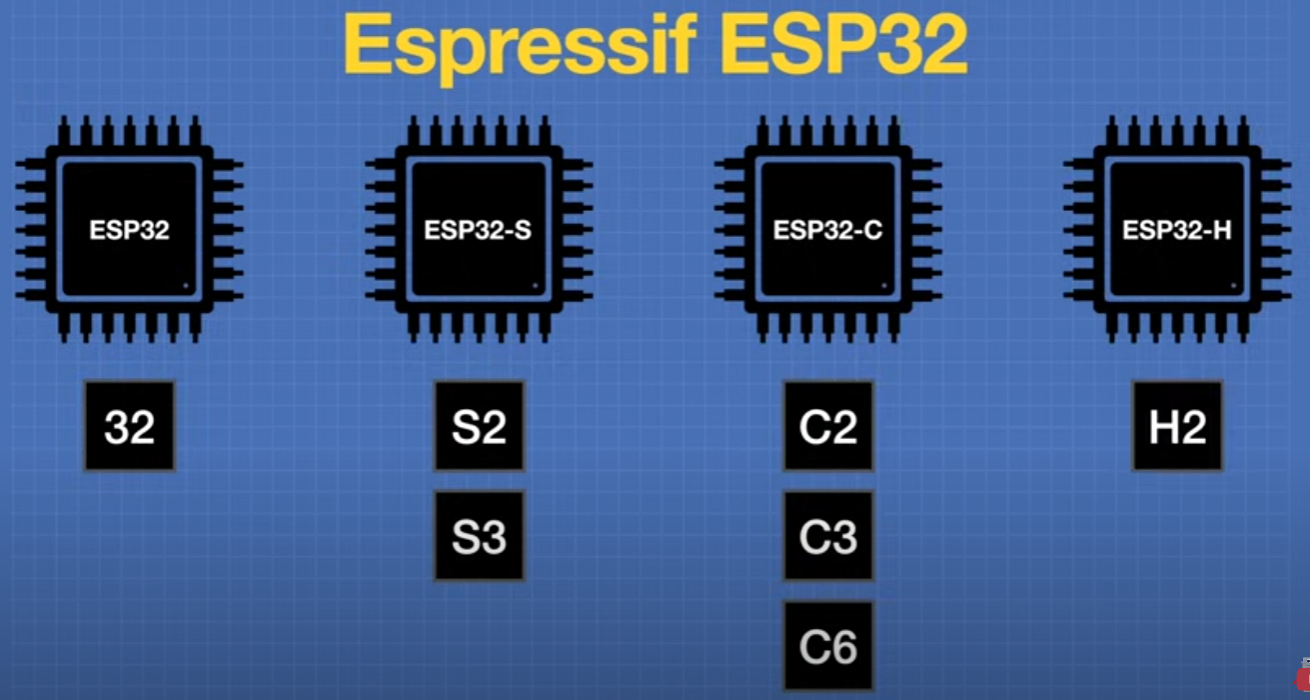
\includegraphics[width=0.8\columnwidth]{Figuras/esp32fam.png}}\\
    \centering{\textbf{Fuente:} \cite{dronebot_esp32_2024}} % Fuente
    \label{fig:esp32fam}
\end{figure}
\newline
Las diferentes versiones de la familia ESP32 varían entre sus características como ser:
\begin{itemize}
    \item \textbf{Microprocesador:} Modelos Xtensa® 32-bit LX6 dual y single core, como tambien el 32-bit single-core RISC-V.
    \item \textbf{SRAM:} A partir de 320 [KB] a 512 [KB].
    \item \textbf{ROM:} A partir de 128 [KB] a 448 [KB].
    \item \textbf{GPIOs:} Distinta cantidad de pines con soporte UART, SPI, I2C, etc.
\end{itemize}
%En la siguiente Figura \ref{fig:esp32comp} se realiza una comparación de características entre los modelos ESP32, ESP32-S2 y ESP32-C3.
%\begin{figure}[!htb]
%    \centering
%    \caption{Comparación de placas de desarrollo ESP32} % Título de figura
%    {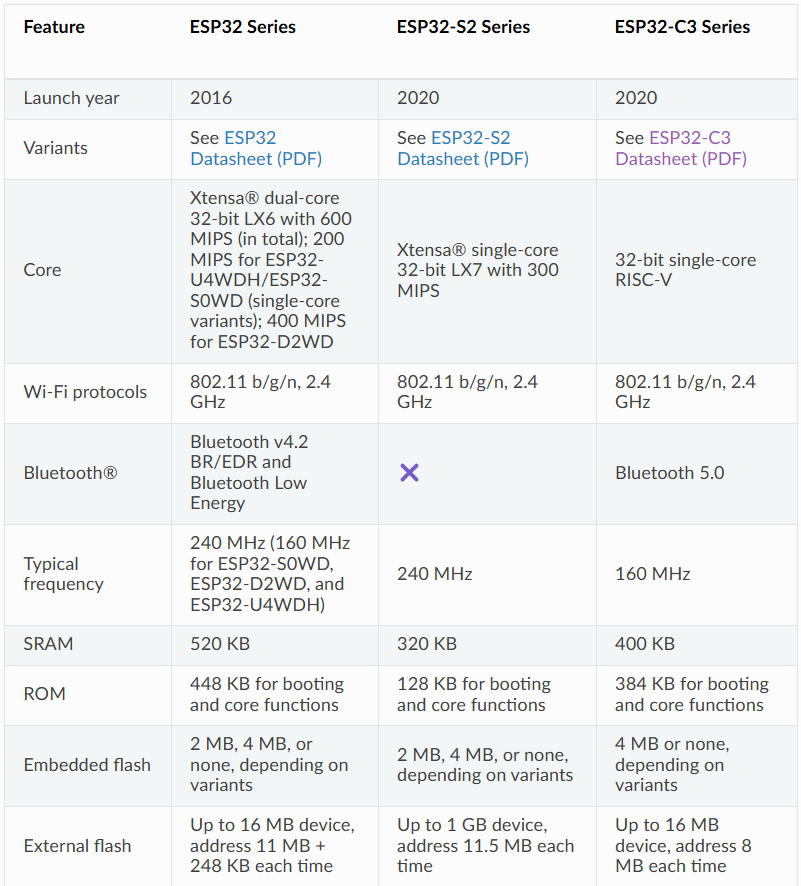
\includegraphics[width=0.9\columnwidth]{Figuras/esp32comp.png}}\\
%    \centering{\textbf{Fuente:} \cite{espressif}} % Fuente
%    \label{fig:esp32comp}
%\end{figure}

El Seeed Studio XIAO ESP32C3 enfocado en tecnologías \acrshort{iot}, en la siguiente Figura \ref{fig:esp32} se observa su asignación de pines.
\begin{figure}[!htb]
    \centering
    \caption{Diagrama de distribución de pines} % Título de figura
    {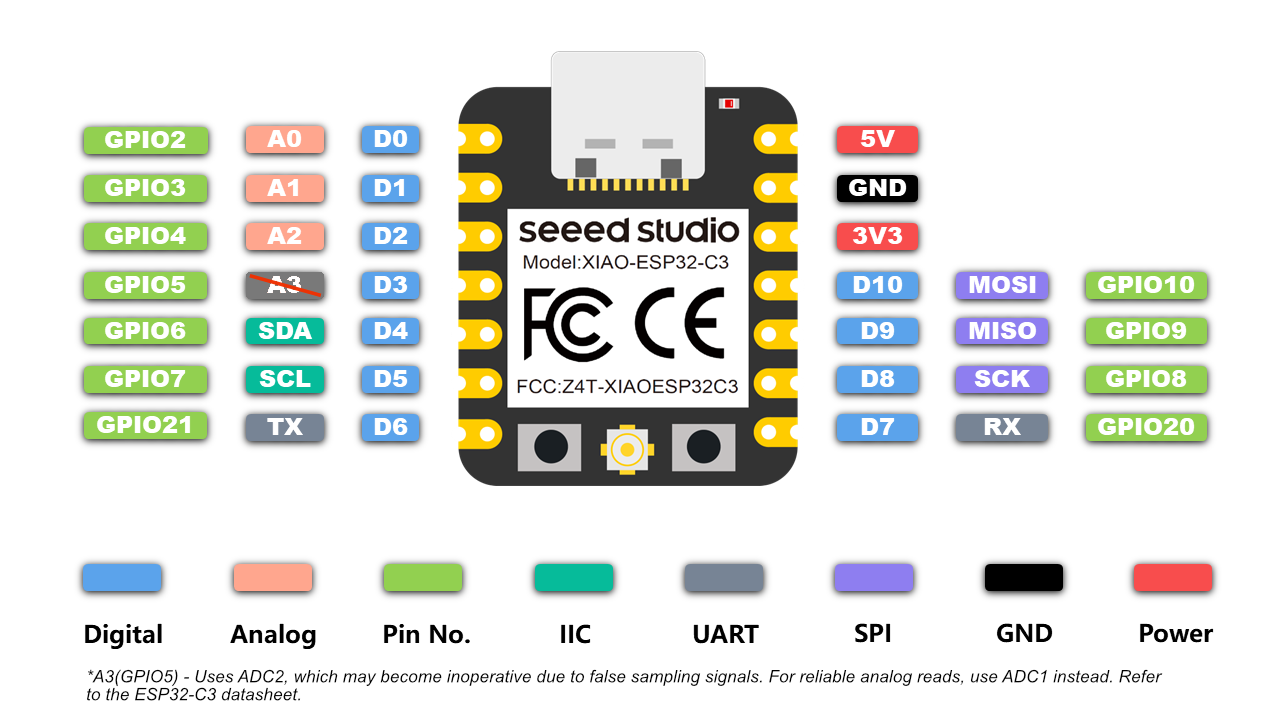
\includegraphics[width=0.8\columnwidth]{Figuras/esp32.png}}\\
    \centering{\textbf{Fuente:} \cite{seeedstudio_xiao_esp32c3}} % Fuente
    \label{fig:esp32}
\end{figure}
\\
Basado en su \textit{datasheet} ubicado en el Anexo \anx{1} se presenta sus siguientes características:
\begin{itemize}
    \item \textbf{Microprocesador:} 32-bit single-core RISC-V.
    \item \textbf{SRAM:} 400 [KB].
    \item \textbf{Wifi:} Cumple el protocolo IEEE 802.11b/g/n.
    \item \textbf{Interfaces:} 2xUART, 1xSPI, 1xI2C, 11xGPIO(PWM) y 4xADC.
    \item \textbf{Tamaño:} Diseño compacto de 21[mm] x 17.8 [mm].
\end{itemize}

\paragraph{STM32}

Es una familia de microcontroladores de 32 bits desarrollada por \textit{STMicroelectronics}. Esta serie se basa en el núcleo ARM Cortex-M, proporciona un alto rendimiento y eficiencia energética con capacidad en tiempo real, procesamiento digital de señales, operaciones de baja potencia y conectividad . Los microcontroladores STM32 incluyen una amplia gama de modelos que varían en la memoria, velocidad de procesamiento, y características periféricas, lo que los hace adecuados para una gran variedad de aplicaciones, desde sistemas embebidos hasta dispositivos \acrshort{iot} \citep{stm32}.

\subsubsection{Protocolos de comunicación seriales}
Los protocolos de comunicación de bajo nivel son estándares que definen cómo los dispositivos intercambian datos directamente a través de medios físicos, como cables o señales inalámbricas, gestionando aspectos como sincronización, codificación y control de errores. 

\paragraph{I2C}
El protocolo \acrfull{i2c} es un estándar de comunicación serial diseñado para la interconexión de dispositivos en sistemas embebidos, permite la comunicación entre un maestro y múltiples esclavos mediante solo dos líneas: \acrshort{sda} para la transferencia de datos y \acrshort{scl} para la sincronización. Este protocolo es ampliamente utilizado en sistemas que requieren la conexión de microcontroladores con sensores, memorias, pantallas y otros periféricos \citep{i2c2012specification}.

\paragraph{Modbus}
Modbus es un protocolo de comunicación creado por Modicon en 1979 para la integración de dispositivos industriales, como PLC y sensores. Su variante Modbus RTU, que utiliza RS-232 o RS-485, es conocida por su formato compacto y confiable, ideal para sistemas SCADA y automatización. Este protocolo permite una comunicación maestro-esclavo eficiente, donde el maestro inicia las solicitudes y los esclavos responden con datos o confirmaciones \cite{modbus2012specification}.

\textbf{RS485}

Es un estándar de comunicación serial desarrollado para entornos industriales, caracterizado por su capacidad de soportar redes multipunto, permitiendo conectar múltiples dispositivos en un mismo bus. Utiliza transmisión diferencial, lo que mejora su inmunidad al ruido y permite alcanzar distancias de hasta 1.200 metros a velocidades de hasta 10 [Mbps]. Es ideal para aplicaciones donde se requiere comunicación robusta en ambientes con interferencias, como en sistemas SCADA y redes de control industrial \cite{rs485spec}.

\textbf{RS232}

Es un estándar de comunicación serial desarrollado en la década de 1960 por la \textit{Electronic Industries Association} para conectar dispositivos como computadoras y periféricos. Utiliza transmisión asíncrona punto a punto, lo que lo hace adecuado para distancias cortas (hasta 15 metros) y velocidades de hasta 115.2 [kbps]. Aunque ha sido reemplazado en muchos casos por interfaces más modernas como USB, RS-232 sigue siendo utilizado en aplicaciones industriales y de depuración debido a su simplicidad y amplia compatibilidad \cite{rs232spec}.

\paragraph{CAN}
CAN es un protocolo de comunicación serial desarrollado por Bosch en la década de 1980, diseñado para redes robustas en automóviles y entornos industriales. Permite la comunicación eficiente entre múltiples nodos sin necesidad de un dispositivo maestro, utilizando un enfoque basado en mensajes con control de acceso mediante prioridad. Su diseño diferencial garantiza alta inmunidad al ruido, ideal para aplicaciones críticas en tiempo real, como control de motores y sistemas de frenado electrónico \cite{canprotocol}.

\subsection{Software requerido para el proyecto}
En esta sección desarrollamos las diferentes herramientas de \textit{software} útiles para la implementación del proyecto.
\subsubsection{Frameworks de desarrollo web}
\paragraph{NextJs}
Next.js es un framework de desarrollo web de código abierto para React, diseñado para la creación de aplicaciones web modernas con renderizado del lado del servidor (SSR) y generación de sitios estáticos (SSG). Su principal ventaja radica en la capacidad de mejorar el rendimiento y la optimización SEO mediante el prerenderizado de páginas. Según \cite{Vercel2020}, Next.js permite a los desarrolladores construir aplicaciones web rápidas y escalables al ofrecer características como la división automática de código, soporte para rutas dinámicas y una estructura de página basada en componentes. Además, Next.js facilita el desarrollo con una configuración mínima, lo que permite un flujo de trabajo simplificado y una experiencia de desarrollo eficiente.
\subparagraph{Principales características}
\begin{itemize}
    \item Obtención de datos simplificación de la obtención de datos mediante \textit{async/await} en componentes del servidor, junto con una API extendida de fetch para memorización de solicitudes y almacenamiento en cache.
    \item Typesript soporte mejorado por Typescript, con una comprobación de tipos más eficiente y una compilación más rápida.
    \item Enrutamiento de sistemas de archivos basado en componentes de servidor que admite diseño, enrutamiento anidado, estado de carga, manejo de errores y más.
    \item Renderizado optimizado, aún más con renderizado estático y dinámico el servidor con Next.js admite streaming en Edge y entornos de Node.js.
    \item Estilos Compatibilidad con \acrfull{css} modules y Tailwind \acrshort{css}.
\end{itemize}

\paragraph{Angular}
Es un \textit{framework} desarrollado por Google ampliamente utilizado para crear aplicaciones web modernas de una sola página. Las funciones integradas de Angular son excelentes y tienen el potencial de hacer que proyectos basados en typescript con un amplio conjunto de herramientas \acrfull{api} y bibliotecas para simplificar y agilizar el flujo de trabajo para el desarrollo \citep{angular}.

\subparagraph{Principales características}
\begin{itemize}
    \item \textbf{Arquitectura basada en componentes:} Los componentes de angular permiten dividir una aplicación en partes mas pequeñas y manejables cada componente debe tener una clase TypeScript, plantilla \acrfull{html} y estilo \acrshort{css}.
    \item \textbf{Inyección de dependencias:} Incluye un sistema de inyección de dependencias manteniendo el código modular, mejora la gestión de servicios y sus dependencias permitiendo aplicaciones más escalables y fáciles de evaluar.
    \item \textbf{Datos en tiempo real:} Gran capacidad para manejar datos en tiempo real, lo que significa que cualquier cambio en los datos se refleja inmediatamente en la vista.
\end{itemize}

\subsubsection{Lenguajes de programación}
Los lenguajes de programación son la herramienta básica de construcción de programas, por lo tanto juegan un papel importante en el desarrollo del proyecto, en esta sección se presenta diferentes lenguajes útiles para la implementación de tecnologías relevantes.
\paragraph{Typescript}
Es un lenguaje de programación que agrega tipado estático a JavaScript esto te permite definir tipos de datos a las funciones y variables es desarrollado y mantenido por Microsoft. Se tiene una gran variedad de entornos de programación que lo utilizan como Node.js, Adobe acrobat y couchDB. Es un lenguaje dinámico basado en un solo hilo multiparadigma que permite estilos de programación orientada objetos, imperativa y funcional. Typescript es un super conjunto de JavaScript lo que significa que todo lo disponible en JavaScript también está disponible en TypeScript y el comportamiento en tiempo de ejecución es el mismo. Puede comprobar si un programa tiene errores antes de su ejecución y lo hace en función de los tipos de valores, lo que lo convierte en un verificador de tipo estático.

Typescript se puede integrar con librerías y plataformas de tiempo real como \textit{websockets}, \acrshort{mqtt}, socket.IO y firebase \citep{typescript}.
\paragraph{C/C++}
El lenguaje de programación C++ es también conocido como el lenguaje de Arduino es la opción predeterminada para programar una placa y conectarla a Arduino Cloud. Este lenguaje es compatible con una alta gama  de placas de desarrollo basadas en ESP32 Y ESP8266.
Al programar en C++ los desarrolladores tienen la ventaja de utilizar \acrshort{api}s lo cual nos permite crear aplicaciones modulares y robustas \citep{arduino_docs}.

\paragraph{Python}
Es un lenguaje de programación interpretado, orientado a la legibilidad de su código, cuenta con programación multi-paradigma y multiplataforma. Desarrollado bajo el concepto de \textit{software} libre, ha ganado una gran y activa comunidad. Cuenta con varios \textit{frameworks} que incrementan su versatilidad, consiguiendo así realizar aplicaciones de análisis de datos, visión artificial, diseño de interfaces, diseño web, análisis de sistemas de control, entre otras \citep{python}.

\subsubsection{Entornos de programación}
Esta herramientas son útiles en el desarrollo de aplicaciones web o funcionalidades para dispositivos.
\paragraph{Visual Studio Code}
Fue creado por la compañía Microsoft y lanzado por primera vez en abril de 2015 cuenta con un editor de código fuente ultrarrápido y versátil que soporta cientos de lenguajes facilitando bastante tareas como autocompletado, depuración interactiva y control de versiones Git. Altamente personalizable adecuado para el desarrollo web. A nivel arquitectónico robusta y extensible combina lo mejor de las tecnologías web, nativas y específicas de lenguajes \citep{vscode_why}.

\paragraph{Arduino IDE}
Es un \acrfull{ide} diseñado para facilitar la programación de microcontroladores Arduino. Este entorno proporciona una interfaz sencilla y accesible para escribir, compilar y cargar código a placas Arduino, permitiendo a los usuarios interactuar con hardware de forma rápida y eficiente. Según \cite{banzi2014arduino}, el Arduino \acrshort{ide} simplifica el proceso de programación al ofrecer una plataforma abierta y flexible, lo que lo convierte en una herramienta popular entre los entusiastas de la electrónica y los desarrolladores de \acrshort{iot}.

\paragraph{PlatformIO}
Es un \acrshort{ide} de código abierto y multiplataforma que ofrece soporte para más de 900 placas de desarrollo y microcontroladores. Es especialmente popular en la comunidad de \acrshort{iot} debido a su capacidad para gestionar proyectos complejos, su integración con herramientas como Visual Studio Code, y su sistema de compilación eficiente. Según \cite{vallet2018platformio}, PlatformIO simplifica la programación y la administración de dependencias, ofreciendo una experiencia de desarrollo más fluida y flexible en comparación con otros entornos como el Arduino \acrshort{ide}, lo que lo convierte en una opción robusta para proyectos de \acrshort{iot} de gran escala.

\paragraph{ESP IDF}
\textit{Espressif IoT Development Framework} es el marco de desarrollo oficial para los microcontroladores ESP32, que proporciona un entorno completo para la programación de aplicaciones \acrshort{iot}. Con ESP-IDF, los desarrolladores pueden aprovechar las capacidades avanzadas de los microcontroladores ESP32, como la conectividad \acrshort{wifi} y Bluetooth, además de la gestión eficiente de recursos. Según \cite{espressif}, ESP-IDF incluye una serie de bibliotecas y herramientas que simplifican el desarrollo de aplicaciones \acrshort{iot}, permitiendo la creación de dispositivos conectados robustos y escalables con características como la conectividad inalámbrica y la integración con la nube.

\subsubsection{Brokers para gestión de datos}

La transmisión y almacenamiento de datos en sistemas \acrshort{iot} generalmente involucra el uso de brokers, que facilitan la comunicación entre dispositivos al gestionar el envío y recepción de mensajes. Los brokers, como \acrshort{mqtt}, actúan como intermediarios entre los dispositivos, asegurando la entrega confiable de datos a través de tópicos y suscripciones. Además, los datos transmitidos suelen almacenarse en bases de datos en la nube o locales, donde pueden ser procesados, analizados y utilizados para la toma de decisiones en tiempo real.

\begin{figure}[!htb]
   \centering
   \caption{Broker MQTT diagrama de funcionamiento}
   {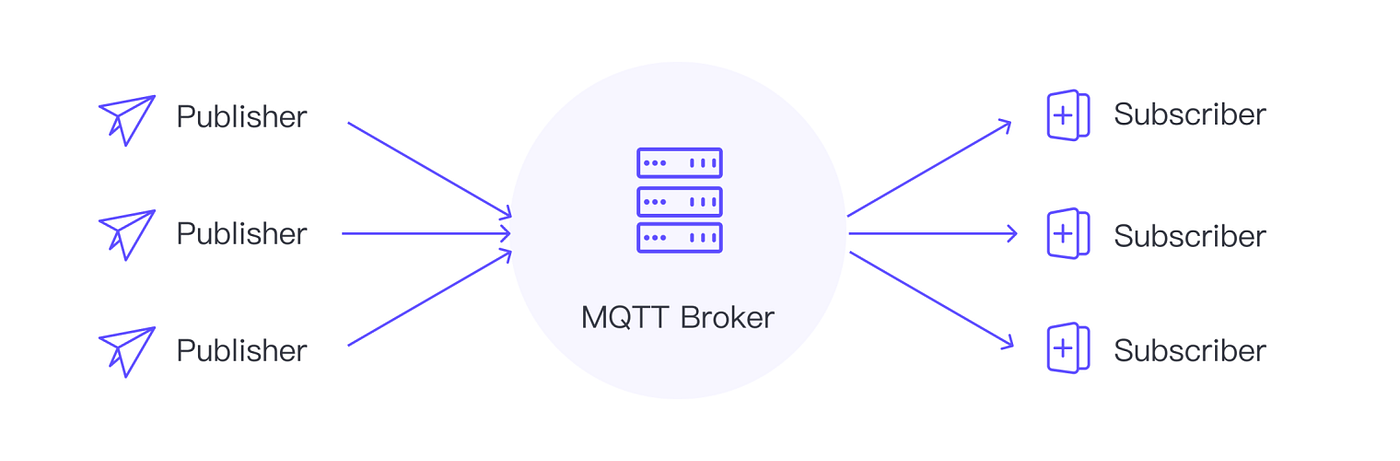
\includegraphics[scale=0.30]{Figuras/MQTT.png}}\\
    \centering{\textbf{Fuente:} EMQT.com }
\end{figure}

\paragraph{EMQX}

EMQX es un broker \acrshort{mqtt} de alto rendimiento y escalabilidad, diseñado para manejar grandes volúmenes de datos y conexiones simultáneas en aplicaciones \acrshort{iot}. Es capaz de gestionar millones de dispositivos y mensajes por segundo, proporcionando una plataforma robusta y eficiente para la transmisión de datos en tiempo real. Según \cite{emq2020}, EMQX soporta múltiples protocolos de comunicación y ofrece características como la seguridad mediante cifrado \acrshort{tls}, autenticación y autorización, además de permitir la integración con sistemas de análisis de datos a través de \acrshort{api}s y otros servicios.

\paragraph{Mosquitto}
Es un broker \acrshort{mqtt} de código abierto ligero y ampliamente utilizado, ideal para dispositivos con recursos limitados y redes con ancho de banda reducido. Ofrece un servicio eficiente de publicación y suscripción para mensajes, permitiendo la integración de \acrshort{iot} en diversas aplicaciones. Según \cite{carleton2018mosquitto}, Mosquitto es altamente eficiente y compatible con una amplia gama de plataformas, lo que lo convierte en una opción popular para la transmisión de datos en tiempo real en sistemas \acrshort{iot} debido a su bajo consumo de recursos y facilidad de implementación.

\paragraph{HiveMQ}
Es un broker \acrshort{mqtt} empresarial diseñado para ofrecer alta escalabilidad, fiabilidad y seguridad en aplicaciones \acrshort{iot} que requieren la transmisión de grandes volúmenes de datos en tiempo real. Su arquitectura distribuida permite manejar millones de conexiones simultáneas, lo que lo convierte en una solución ideal para sistemas \acrshort{iot} a gran escala. Según \cite{wolf2016hivemq}, HiveMQ es compatible con protocolos estándares y ofrece características avanzadas como la integración con sistemas de \textit{backend}, alta disponibilidad, y herramientas para la administración de datos, lo que lo convierte en una opción robusta para empresas que requieren confiabilidad y rendimiento.

\subsubsection{Plataformas de almacenamiento de datos}
Son aquellos espacios centralizados que consisten en almacenar diferentes tipos de datos en la nube y permiten ser accedidos desde múltiples fuentes o ubicaciones, se presenta los siguientes como principales opciones para uso en el proyecto.
\paragraph{MongoDb}
Es una base de datos no relacional orientada a documentos que almacena datos en formato \acrfull{json}, lo que la hace flexible y escalable para aplicaciones \acrshort{iot} que generan grandes volúmenes de datos. Su estructura de documentos permite almacenar información diversa y no estructurada, facilitando la integración con sistemas \acrshort{iot} que requieren rapidez en el acceso a datos en tiempo real. Según \cite{chodorow2013mongodb}, MongoDB es ideal para manejar datos distribuidos y a gran escala debido a su capacidad de replicación y \textit{sharding}, lo que la convierte en una opción popular para proyectos que requieren alto rendimiento y disponibilidad.

\paragraph{Firebase}
Firebase es una plataforma de desarrollo móvil y web que ofrece una amplia gama de herramientas para la gestión de bases de datos en tiempo real, autenticación, almacenamiento y notificaciones \textit{push}. Su base de datos en tiempo real permite a los desarrolladores sincronizar datos de forma instantánea entre los usuarios y dispositivos, lo que la convierte en una opción ideal para aplicaciones \acrshort{iot} que requieren actualizaciones constantes en tiempo real. Según \cite{moffatt2018firebase}, Firebase simplifica el desarrollo de aplicaciones escalables, proporcionando una infraestructura robusta para la gestión de datos y la integración de servicios en la nube.

\paragraph{InfluxDb}
InfluxDB es una base de datos de series temporales diseñada específicamente para almacenar y analizar grandes volúmenes de datos con una alta frecuencia de escritura, lo que la hace ideal para aplicaciones \acrshort{iot} que requieren monitoreo en tiempo real. Su capacidad para manejar datos con marcas de tiempo la convierte en una herramienta eficiente para almacenar métricas y eventos, facilitando el análisis de datos históricos y la detección de patrones. Según \cite{jovanovic2018influxdb}, InfluxDB ofrece una estructura de datos optimizada para consultas rápidas y es ampliamente utilizada en sistemas de monitoreo y análisis de datos en entornos industriales y de \acrshort{iot} debido a su rendimiento y escalabilidad.

\subsubsection{Software de diseño electrónico}
La parte del diseño electrónico se enfoca en enunciar las herramientas consideraras para la creación de circuitos y sistemas electrónicos que cumplen funciones específicas, en el diseño de un sistema de monitoreo remoto este proceso incluye la conceptualización, simulación, y finalmente la implementación en \textit{hardware}, como \acrfull{pcb}. En resumen se muestran las herramientas y software llamados \acrfull{eda} que facilitan el diseño y la optimización de sistemas electrónicos necesarios para el proyecto.

\paragraph{EASYEDA}

EasyEDA es una herramienta en línea para el diseño de circuitos electrónicos y la creación de placas \acrshort{pcb}s que permite a los ingenieros y diseñadores electrónicos desarrollar, simular y producir sus proyectos de manera eficiente. Esta plataforma ofrece una interfaz intuitiva y herramientas de simulación para verificar el comportamiento del circuito antes de la fabricación, lo que facilita el proceso de diseño. Según \cite{leung2020easyeda}, EasyEDA se destaca por su integración con servicios de fabricación de \acrshort{pcb}s y su compatibilidad con otros programas de diseño electrónico, lo que la convierte en una opción accesible tanto para principiantes como para expertos en diseño de \textit{hardware}.

\paragraph{KiCad}
Es un entorno de \textit{software} libre \acrshort{eda} usado para el diseño de circuitos eléctricos, muy flexible y adaptable, en el que se pueden crear y editar un gran número de componentes. KiCad permite el diseño de \acrshort{pcb}s modernos de forma sencilla e intuitiva. La aplicación se ejecuta en Windows, Linux y macOS y tiene licencia GNU GPL v3 \citep{kicad}. 

\paragraph{Proteus}
El programa Proteus, de \textit{Labcenter Electronics}, permite cubrir todas las fases que van desde la idea hasta la implementación de la misma en forma de placa de circuito impreso o \acrshort{pcb}: captura de esquema, simulación de funcionamiento y diseño. Si bien no es la única herramienta del mercado que permite realizar estas tareas, la posibilidad de llevar a cabo simulaciones interactivas del circuito a diseñar y de incluir dispositivos microcontroladores en estas simulaciones le confieren a Proteus un valor añadido del que carecen otros paquetes de programas similares \citep{prieto2018proteus}.

\subsubsection{Software de diseño mecánico}
En la industria se ha implementado diversas herramientas como las \acrfull{cad}, \acrfull{cae} y \acrfull{cam}, son aplicaciones que facilitan el diseño mecánico computacional logrando así agilizar el proceso de manufactura, ofreciendo funcionalidades como la creación de piezas, planos, ensamblaje, análisis de esfuerzos, etc.
\paragraph{Solidworks}
Es un software de diseño \acrshort{cad}, \acrshort{cae} y \acrshort{cam} desarrollado por Dassault Systèmes, conocido por su interfaz potente, pero fácil de usar, es el estándar de referencia en el sector de modelado 3D. Nos permite realizar todas las tareas de diseño y simulación, como también la generación de documentación como planos e informes, puesto que tiene gran cantidad de distribuciones \citep{solidworks}.